\section{Řešení rovnic jednobodové kinetiky}

\subsection{Řešení bez vlivu zpožděných neutronů}

Řešení rovnice bez započtení zpožděných neutronů je triviální (jedná se pouze o jednu lineární diferenciální rovnici prvního řádu) a už zde bylo zmíněno. Pro zopakování, řešíme rovnici:

$$ \dfrac{dN}{dt} = \dfrac{\rho (t)}{\Lambda} N(t) $$

s počáteční podmínkou $N(0) = N_0$ (ustálený stav).\\

\subsubsection{Konstatní reaktivita}

Při $\rho = \text{konst.}$ vede rovnice na exponenciální řešení:

\begin{equation}
  \boxed{
  N(t) = N_0 \exp \left ( \dfrac{\rho_0}{\Lambda} t \right ).
  \label{kinetika_reseni}}
\end{equation}

\subsection{Řešení s vlivem zpožděných neutronů -- postup}

Řešíme soustavu lineárních diferenciálních rovnic:

$$ \dfrac{dN}{dt} = \dfrac{\rho(t) - \beta_{\text{ef}}}{\Lambda} N(t) + \sum_{i=1}^m \lambda_i C_i(t), $$

$$ \dfrac{dC_i}{dt} = -\lambda_i C_i(t) + \dfrac{\beta_{\text{ef},i}  N(t)}{\Lambda}. $$

s počátečními podmínkami (ustálený stav) $N(0) = N_0$ a $C_i(0) = C_{i,0}$. Tento stav lze předpokládat, pokud se reaktor nachází dostatečně dlouhou dobu v ustáleném stavu (při konstantním výkonu), potom je i koncentrace jader $C_i$ konstantní. Tuto koncentraci lze získat z druhé rovnice z doby před $t=0$:

$$ 0 = -\lambda_i C_{i,0} + \dfrac{\beta_{\text{ef},i}  N_0}{\Lambda} \rightarrow C_{i,0} = \dfrac{\beta_{\text{ef},i}  N_0}{\Lambda \lambda_i}. $$

Aplikujme na obě rovnice LT, dostaneme:

$$ s \tilde{N}(s) - N_0 = \dfrac{\mathcal{L}[\rho(t) N(t)](s)}{\Lambda} - \dfrac{\beta_{\text{ef}} \tilde{N}(s)}{\Lambda} + \sum_{i=1}^m \lambda_i \tilde{C_i}(s), $$

$$ s \tilde{C_i}(s) - C_{i,0} = -\lambda_i \tilde{C_i}(s) + \dfrac{\beta_{\text{ef},i}  \tilde{N}(s)}{\Lambda}. $$

Do druhé rovnice můžeme rovnou dosadit za $C_{i,0}$ (známe z počátečních podmínek, $N_0$ zachováváme, to získáme z normalizace výkonu), čímž získáváme soustavu algebraických rovnic:

$$ s \tilde{N}(s) - N_0 = \dfrac{\mathcal{L}[\rho(t) N(t)](s)}{\Lambda} - \dfrac{\beta_{\text{ef}} \tilde{N}(s)}{\Lambda} + \sum_{i=1}^m \lambda_i \tilde{C_i}(s), $$

$$ s \tilde{C_i}(s) - \dfrac{\beta_{\text{ef},i}  N_0}{\Lambda \lambda_i} = -\lambda_i \tilde{C_i}(s) + \dfrac{\beta_{\text{ef},i}  \tilde{N}(s)}{\Lambda}. $$

Pokračujeme tak, že z druhé rovnice vyjádříme $\lambda_i \tilde{C_i}(s)$:

$$ \lambda_i \tilde{C_i}(s) = \dfrac{\beta_{\text{ef},i} \lambda_i \tilde{N}(s) + \beta_{\text{ef},i}N_0}{\Lambda(\lambda_i + s)} $$

a dosadíme do první rovnice (s vynásobením $\Lambda$):

$$ \Lambda (s \tilde{N}(s) - N_0) = \mathcal{L}[\rho(t) N(t)](s) - \beta_{\text{ef}} \tilde{N}(s) + \sum_{i=1}^m \dfrac{\beta_{\text{ef},i} \lambda_i \tilde{N}(s)}{\lambda_i + s} + \sum_{i=1}^m \dfrac{\beta_{\text{ef},i}N_0}{\lambda_i + s}. $$

Nyní rozepíšeme $\beta_{\text{ef}}$ do sumy přes $\beta_{\text{ef},i}$ a rozšíříme přes $\lambda_i + s$. Po vynásobení se něco požere:

$$ \Lambda (s \tilde{N}(s) - N_0) = \mathcal{L}[\rho(t) N(t)](s) - \sum_{i=1}^m \dfrac{\beta_{\text{ef},i} \tilde{N}(s)}{\lambda_i + s}(\lambda_i + s) + \sum_{i=1}^m \dfrac{\beta_{\text{ef},i} \lambda_i \tilde{N}(s)}{\lambda_i + s} + \sum_{i=1}^m \dfrac{\beta_{\text{ef},i}N_0}{\lambda_i + s}, $$

$$ \Lambda (s \tilde{N}(s) - N_0) = \mathcal{L}[\rho(t) N(t)](s) - \sum_{i=1}^m \dfrac{\beta_{\text{ef},i} \lambda_i \tilde{N}(s)}{\lambda_i + s} - \sum_{i=1}^m \dfrac{\beta_{\text{ef},i} s \tilde{N}(s)}{\lambda_i + s} + \sum_{i=1}^m \dfrac{\beta_{\text{ef},i} \lambda_i \tilde{N}(s)}{\lambda_i + s} + \sum_{i=1}^m \dfrac{\beta_{\text{ef},i}N_0}{\lambda_i + s}, $$

$$ \Lambda (s \tilde{N}(s) - N_0) = \mathcal{L}[\rho(t) N(t)](s) - \sum_{i=1}^m \dfrac{\beta_{\text{ef},i} s \tilde{N}(s)}{\lambda_i + s} + \sum_{i=1}^m \dfrac{\beta_{\text{ef},i}N_0}{\lambda_i + s}. $$

Z PS rovnice vytáhneme $(s \tilde{N}(s) - N_0)$:

$$ \Lambda (s \tilde{N}(s) - N_0) = \mathcal{L}[\rho(t) N(t)](s) - \left [ \sum_{i=1}^m \dfrac{\beta_{\text{ef},i}}{\lambda_i + s}(s \tilde{N}(s) - N_0) \right ]$$

a po převedení sumy na LS:

$$ \left ( \Lambda + \sum_{i=1}^m \dfrac{\beta_{\text{ef},i}}{\lambda_i + s} \right ) (s \tilde{N}(s) - N_0) = \mathcal{L}[\rho(t) N(t)](s). $$

Nyní je konečně možné vyjádřit $\tilde{N}(s)$:

$$ \tilde{N}(s) = \dfrac{\mathcal{L}[\rho(t) N(t)](s)}{s \left ( \Lambda + \sum_{i=1}^m \dfrac{\beta_{\text{ef},i}}{\lambda_i + s} \right )} + \dfrac{N_0}{s}. $$

Nyní pro zjednodušení zápisu zavedeme tzv. \textbf{přenosovou funkci nulového reaktoru} $\tilde{G_0}(s)$ vztahem:

\begin{equation}
  \boxed{
  \tilde{G_0}(s) \equiv \dfrac{1}{s \left ( \Lambda + \sum_{i=1}^m \dfrac{\beta_{\text{ef},i}}{\lambda_i + s} \right )}.
  \label{prenosova_funkce}
  }
\end{equation}

Potom platí:

$$ \tilde{N}(s) = \tilde{G_0}(s) \cdot \mathcal{L}[\rho(t) N(t)](s) + \dfrac{N_0}{s}. $$

Teď už pouze zbývá provést inverzní LT. Ale to je vopruz, takže budeme postupovat obráceně. Z vět o LT konvoluce a konstanty (0.~kapitola) je jasné, že:

$$ \tilde{N}(s) = \tilde{G_0}(s) \cdot \mathcal{L}[\rho(t) N(t)](s) + \dfrac{N_0}{s} $$
$$ \Leftrightarrow $$
$$ N(t) = G_0(t) * [\rho(t) N(t)] + N_0. $$

Po aplikaci definice konvoluce (opět 0.~kapitola) získáváme \textbf{Rovnici jednobodové kinetiky v integrálním tvaru}:

\begin{equation}
  \boxed{
  N(t) = N_0 + \int_0^t G_0(t-t') \rho(t') N(t')dt'.
  \label{integralni_kinetika}
  }
\end{equation}

To je všechno pěkný, ale musíme ještě znát obraz přenosové funkce $G_0(t)$. Zde musíme vycházet z definice $\tilde{G_0}(s)$, kterou převedeme na parciální zlomky a aplikací vět z 0.~kapitoly není obtížné nalézt původní funkci $G_0(t)$. To ale dělat nebudeme, musí nám stačit vědět, že něco takového je možné\footnote{:)}. Platí totiž:

$$ \tilde{G_0}(s) = \dfrac{\varphi(s)}{\Psi(s)} = \sum_{n=0}^m \dfrac{A_n}{s-s_n}, $$

kde $\varphi(s)$ je libovolný polynom, $\Psi(s)$ je polynom řádu $m$ a $s_n$ jsou jeho kořeny. $A_n$ jsou konstanty získané dle:

$$ A_n = \dfrac{\varphi(s_n)}{\Psi'(s_n)}. $$

Po převodu (suma lomených výrazů se zpět transformuje na sumu exponenciál) dostaneme:

\begin{equation}
  \boxed{
  G_0(t) = \sum_{n=0}^m A_n e^{s_n t}.
  \label{prenosova_funkce_reseni}
  }
\end{equation}

\textbf{Kuchařka s postupem:}

Následní text je pouze matematická kuchařka, jak získat koeficienty $A_n$ a $s_n$. Definovaný vztah \eqref{prenosova_funkce} rozšíříme výrazem $\prod_{n=1}^m (s+\lambda_n)$, čímž se nám ve jmenovateli něco požere:

$$ \tilde{G_0}(s) \equiv \dfrac{\prod_{n=1}^m (s+\lambda_n)}{s \left ( \Lambda \prod_{n=1}^m (s+\lambda_n)  + \sum_{n=1}^m \beta_{\text{ef},n}\prod_{k=1, k \neq n}^m(\lambda_k + s) \right )}. $$

Jaké budou kořeny polynomu ve jmenovateli? První je jasný, tj. $s_0 = 0$. Výraz v hranaté závorce je natuty kladný $\rightarrow$ zbylé kořeny nemohou být kladné $\rightarrow$ zbylé kořeny jsou určitě záporné, tj. $s_1, s_2, ..., s_n < 0$.\\

Abychom získali konstanty $A_n$, je vhodné si polynomy upravit do lepšího tvaru. Z MAA1 víme:

$$ \Psi(s) = K \cdot \prod_{n=0}^m (s-s_n) $$

a jelikož známe první kořen $s_0 = 0$:

$$ \Psi(s) = K \cdot s \prod_{n=1}^m (s-s_n) $$

Chybí nám už pouze získat konstantu $K$. Tu získáme z řešení limity $\lim_{s \to \infty} s \cdot \tilde{G_0}(s)$. Z definice přenosové funkce \eqref{prenosova_funkce} platí:

$$ \lim_{s \to \infty} s \cdot \left [ \dfrac{1}{s \left ( \Lambda + \sum_{n=1}^m \dfrac{\beta_{\text{ef},n}}{\lambda_n + s} \right )} \right ] = \dfrac{1}{\Lambda} $$

a z námi upraveného tvaru pro polynom $\Psi(s)$ (ten, ve kterém se objevuje konstanta $K$) zase platí:

$$ \lim_{s \to \infty} s \cdot \left [ \dfrac{\prod_{n=1}^m (s+\lambda_n)}{K \cdot s \prod_{n=1}^m (s-s_n)} \right ] = \dfrac{1}{K} $$

Je tedy jasné, že:

$$ K = \Lambda, $$

a tedy:

$$ \tilde{G_0}(s) = \dfrac{\prod_{n=1}^m (s+\lambda_n)}{\Lambda \cdot s \prod_{n=1}^m (s-s_n)}. $$

Pro ty co se ztratili v tom, o co se vlastně snažíme. Pokoušíme se nalézt konstanty $A_n$, které jsme si pro připomenutí definovali jako:

$$ \tilde{G_0}(s) = \dfrac{\varphi(s)}{\Psi(s)} = \sum_{n=0}^m \dfrac{A_n}{s-s_n}, $$

$$ A_n = \dfrac{\varphi(s_n)}{\Psi'(s_n)}, $$

kde v našem značení:

$$ \Psi(s) = \Lambda \cdot s \prod_{n=1}^m (s-s_n). $$

Funkci $\Psi(s)$ musíme derivovat, což je jednoduché, jelikož se jedná o produkt. Pro jeho derivaci platí:

$$ \dfrac{d}{dx} \left ( \prod_{i=1}^k f_i(x) \right ) = \sum_{i=1}^k \left ( \dfrac{f_i'(x)}{f_i(x)} \prod_{j=1,j \neq i}^k f_j(x) \right ). $$

Už je pozdě a je zbytečné rozepisovat postupy, zkrátka platí, že:

$$ \Psi'(s) = \Lambda \prod_{n=1}^m (s-s_n) + \Lambda \cdot s \sum_{n=1}^m \prod_{k=1, k \neq n}^m (s-s_k). $$

Při dosazení prvního kořene $s_0 = 0$ je řešení triviální, při dosazování zbylých kořenů je první člen vždy nulový a u druhého členu vypadne suma. Tedy:

$$ \Psi'(s_0) = \Lambda \cdot \prod_{i=1, i \neq n}^m (-s_i), \: \: \: n = 0, $$

$$ \Psi'(s_n) = \Lambda \cdot s_n \prod_{i=1, i \neq n}^m (s_n-s_i), \: \: \: \forall \: n \in \widehat{m}. $$

Rovněž platí (a bude se hodit):

$$ \sum_{n=0}^m A_n = \dfrac{1}{\Lambda}. $$

\subsection{Analytické řešení s vlivem zpožděných neutronů}

Vycházíme z řešení rovnice jednobodové kinetiky v integrálním tvaru \eqref{integralni_kinetika}. Rovnice je analyticky řešitelná pouze pro 3 různé případy $\rho$:

\begin{itemize}
  \item impuls $\rightarrow$ impulsní charakteristika,
  \item konstanta $\rightarrow$ přechodová charakteristika,
  \item periodická závislost $\rightarrow$ frekvenční charakteristika.
\end{itemize}

\subsubsection{Impulsní charakeristika}

Jde tedy o případ, kdy do kritického systému zasáhneme kladnou/zápornou reaktivitu ve tvaru impulsu. Reálně nemůže nastat, ale matematicko-idealisticky lze $\rho$ vyjádřit pomocí Dirackovy $\delta$ funkce:

$$ \rho(t) = \rho_0 \delta (t). $$

Dále tedy řešíme rovnici \eqref{integralni_kinetika}:

$$ N(t) = N_0 + \int_0^t G_0(t-t') \rho(t') N(t')dt', $$

$$ N(t) = N_0 + G_0(t) \rho_0 N_0. $$

Nás ale zajímá relativní změna $\dfrac{\Delta N}{N_0}$, přičemž za $G_0(t)$ dosadíme z \eqref{prenosova_funkce_reseni}:

\begin{equation}
  \boxed{
  \dfrac{\Delta N}{N_0} = \rho_0 G_0 (t) = \rho_0 \sum_{n=0}^m A_n e^{s_n t}.
  \label{impulsni_charakteristika}}
\end{equation}

Ohledně znamének v kořenech:

\begin{itemize}
  \item $s_0 = 0$,
  \item $s_n < 0 \: \: \: \forall \: n \in \widehat{m}$.
\end{itemize}

Díky zápornosti kořenů jsou exponenciály ve výrazu \eqref{impulsni_charakteristika} klesající, tudíž i průběh relativní změny četnosti je klesající. Nejde ovšem k nule a v $t=0$ nejde k nekonečnu! Dále by nás tedy mohly zajímat limitní případy pro $t \rightarrow 0^+$ a $t \rightarrow \infty$. Řešíme přes limity:

$$ \lim_{t \to 0^+} \dfrac{\Delta N}{N_0} = \rho_0 \sum_{n=0}^m A_n = \dfrac{\rho_0}{\Lambda} \doteq \dfrac{\rho_0}{\ell}, $$

$$ \lim_{t \to \infty} \dfrac{\Delta N}{N_0} = \rho_0 \lim_{s \rightarrow 0} s \tilde{G_0}(s) = \dfrac{\rho_0}{\Lambda + \sum_{i = 1}^m \dfrac{\beta_{\text{ef},i}}{\lambda_i}} \doteq \dfrac{\rho_0}{\ell^*}. $$

Průběh relativní změny četnosti při vnesení kladné i záporné reaktivity zobrazuje obrázek \ref{fig_impulsni}.

\begin{figure}[H]
  \centering
  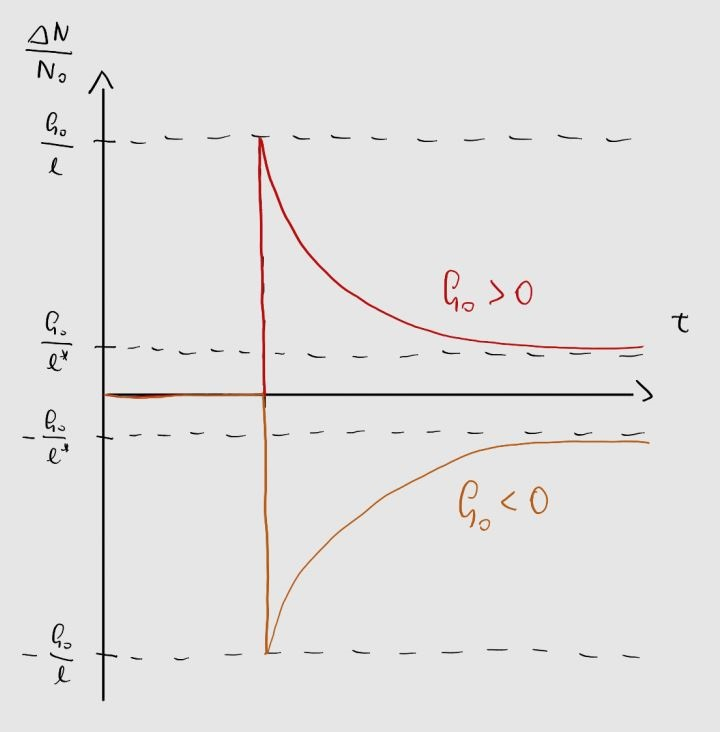
\includegraphics[width=0.6\textwidth]{img/impulsni.jpg}
  \caption{Závislost relativní změny četnosti neutronů pro impulsní charakteristiku.}
  \label{fig_impulsni}
\end{figure}

Je tedy jasné, že v čase $t=0$ je relativní změna četnosti neutronů ovlivněna okamžitými neutrony a v čase $t \rightarrow \infty$ zpožděnými neutrony. V reálu se u vysokých vložených reaktivit (TRIGA) výrazně projevují zpětné vazby. Výrazy platí pro záporné i kladné vnesené reaktivity.

\subsubsection{Přechodová charakteristika}

Jde o případ, kdy je vložená reaktivita konstantní, tedy:

$$\rho(t) = \rho_0$$

Lze aplikovat i v reálu (pád tyče), i když ve skutečnosti to tak není (tyč padá nějakou tu dobu). Pro řešení vycházíme ještě z doby před zavedením integrální podoby jednobodové kinetiky\footnote{Tady si pro další usnadnění života přepíšu proměnou v LT pomocí $z$, aby se mi nepletlo s obecným řešením.}:

$$ \tilde{N}(z) = \dfrac{N_0}{z} + \tilde{G_0}(z) \cdot \mathcal{L}[\rho(t) N(t)](z), $$

$$ \tilde{N}(z) = \dfrac{N_0}{z} + \rho_0 \tilde{G_0}(z) \tilde{N}(z).$$

Nás zajímá relativní četnost $\dfrac{\tilde{N}(z)}{N_0}$ a zároveň za $\tilde{G_0}(z)$ dosadíme z \eqref{prenosova_funkce}, tedy:

\begin{equation}
  \boxed{
  \dfrac{\tilde{N}(z)}{N_0} = \dfrac{1}{z \left ( 1-\rho_0 \tilde{G_0}(z) \right )} = \dfrac{\Lambda + \sum_{i = 1}^m \dfrac{\beta_{\text{ef},i}}{z + \lambda_i}}{z \left ( \Lambda + \sum_{i = 1}^m \dfrac{\beta_{\text{ef},i}}{z + \lambda_i} \right ) - \rho_0}.
  \label{prechodova_charakteristika_LT}}
\end{equation}

Rovnice \eqref{prechodova_charakteristika_LT} se dá transformovat úplně stejně, jako v minulé kapitole $\rightarrow$ převedu na parciální zlomky:

$$ \dfrac{\tilde{N}(z)}{N_0} = \sum_{n=0}^m \dfrac{C_n}{z-z_n}, $$

\begin{equation}
  \boxed{
  \dfrac{N(t)}{N_0} = \sum_{n=0}^m C_n e^{z_n t}.
  \label{prechodova_charakteristika}}
\end{equation}

Zaměříme-li se na znaménka koeficientů $C_n$ a $z_n$, tak:

\begin{itemize}
  \item $z_0$ má stejné znaménko jako $\rho_0$,
  \item $z_n < 0 \: \: \: \forall \: n \in \widehat{m}$,
  \item $C_0 > 0$,
  \item $C_n$ mají opačná znaménka než $\rho_0, \: \: \: \forall \: n \in \widehat{m}$.
\end{itemize}

Vztah mezi kořeny $z_n$ v závislosti na reaktivitě zobrazuje graf na obrázku \ref{fig_zn-rho}.

\begin{figure}[H]
  \centering
  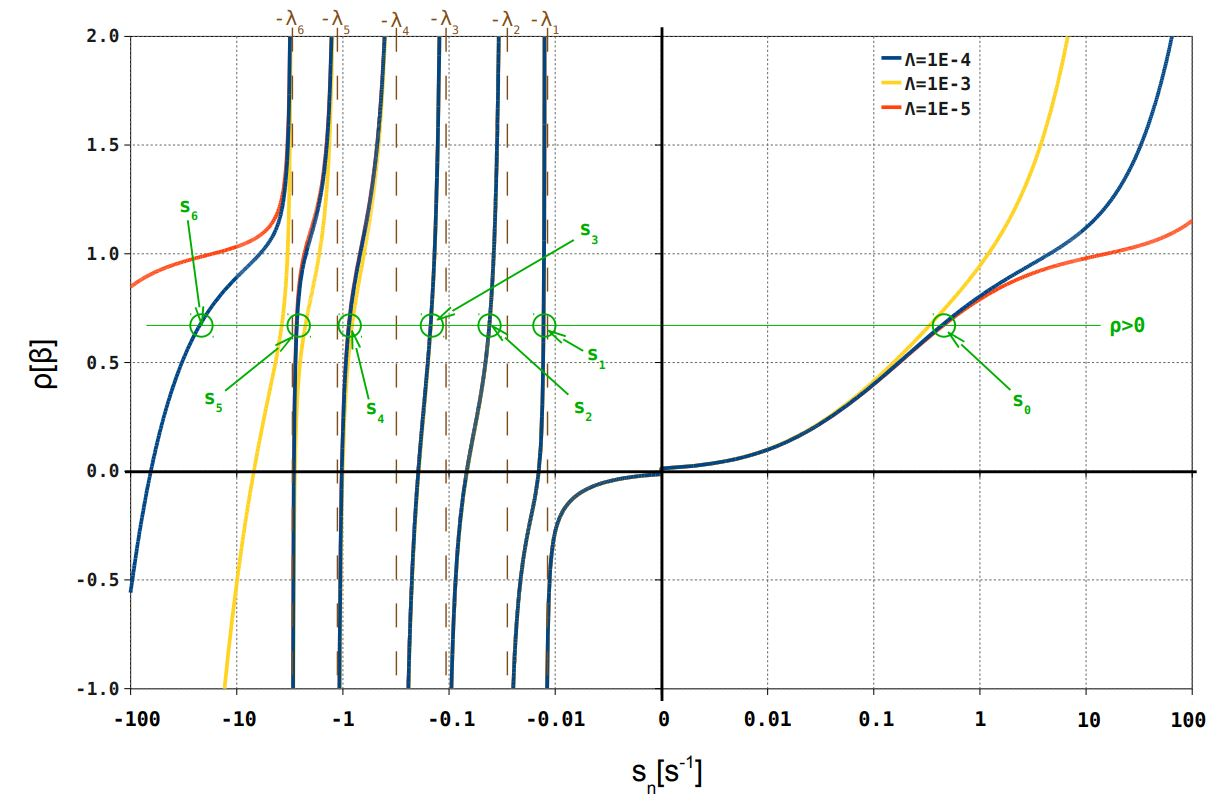
\includegraphics[width=1\textwidth]{img/zn-rho.jpg}
  \caption{Vztah mezi kořeny $z_n$ (zde $s_n$) a reaktivitou $\rho_0$ v přechodové charakteristice.}
  \label{fig_zn-rho}
\end{figure}

Pro $\rho_0 < 0$ bude relativní četnost v čase exponenciálně klesat (což bude ovlivněno největším $|z_n|$, což je závislé na $\Lambda$ $\rightarrow$ s menším $\Lambda$ očekáváme strmější nástup).\\

Pro $\rho_0 > 0$ po chvíli převládne kladné $z_0$ s $C_0$ a relativní četnost exponenciálně poroste. Do tohoto zlomového okamžiku bude relativní četnost také růst, ale s jiným průběhem.

Průběh relativní četnosti při vnesení kladné i záporné reaktivity zobrazuje obrázek \ref{fig_prechodova}.

\begin{figure}[H]
  \centering
  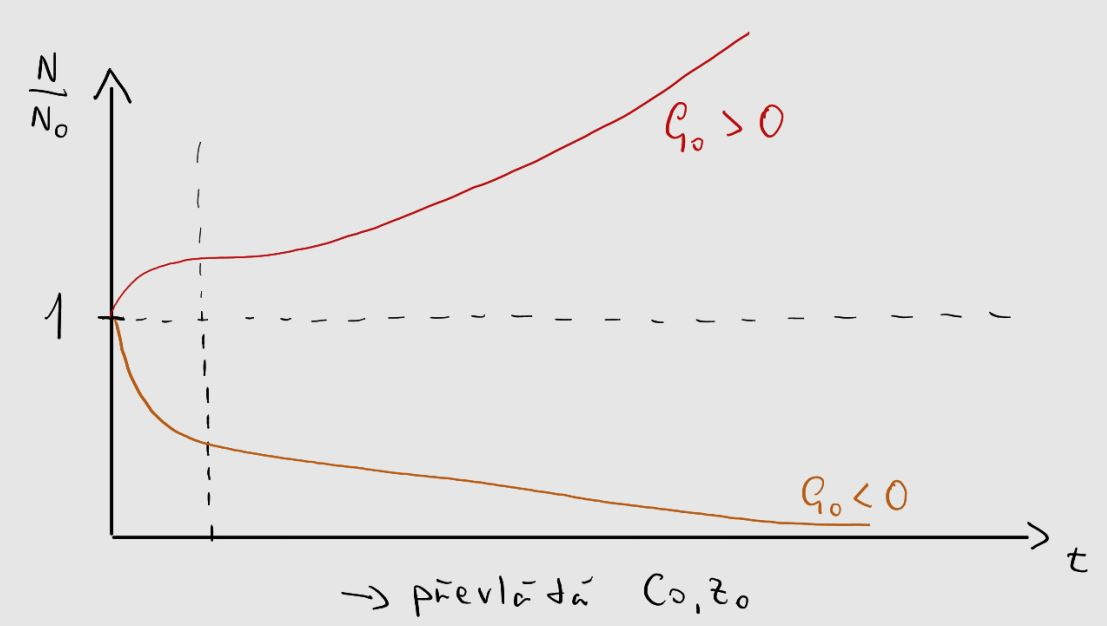
\includegraphics[width=0.7\textwidth]{img/prechodova.jpg}
  \caption{Závislost relativní četnosti neutronů pro přechodovou charakteristiku.}
  \label{fig_prechodova}
\end{figure}

\textbf{Ustálená perioda reaktoru}

Po vymizení všech členů, kdy bude vývoj ovlivněn pouze členy $z_0$ a $C_0$, bude možné popsat relativní četnost pomocí právě jedné exponenciály:

$$ \dfrac{N(t)}{N_0} = C_0 e^{z_0 t}. $$

Tento vztah je možné využít při vymizení většiny skupin zpožděnek, v tzv. \textbf{asymptotické oblasti} kdy už převládá pouze nejdelší ze skupin s $\tau_1 \approx 80$~s. Poté je možné stanovit tzv. \textbf{ustálenou periodu reaktoru} jako:

$$ T_e = \dfrac{1}{z_0}, $$

což při dosazení do vztahu, který jsme získali v minulé kapitole (při hledání kořenů $z_n$ pomocí položení jmenovatele nule)\footnote{Platí pro každé $z_n$, tedy i pro $z_0$}:

\begin{equation}
  \rho_0 = z_0 \left ( \Lambda + \sum_{i = 1}^m \dfrac{\beta_{\text{ef},i}}{z_0 + \lambda_i} \right )
  \label{rho0-z0}
\end{equation}

dává tzv. \textbf{in-hour equation}, tedy vztah, který dává do souvislosti reaktivitu a peroidu\footnote{Tohle jsme dělali právě na ERF, kdy jsme vložili kladnou reaktivitu a čekali, až se četnost začne zvyšovat podle jedné exponenciály. U té jsme poté určili její koeficient (směrnici v log měřítku) a po zadání do tohodle vztahu jsme zjistili hledanou kladnou reaktivitu.}:

\begin{equation}
  \boxed{
  \rho_0 = \dfrac{\Lambda}{T_e} + \sum_{i=1}^{m} \dfrac{\beta_{\text{ef},i}}{1 + \lambda_i T_e}.
  \label{in-hour}}
\end{equation}

\small

\textbf{Př. 3 - přechodová charakteristika pro 1 skupinu zpožděnek:}

Vyzkoušíme si přechodovou charakteristiku na jedné skupině zpožděných neutronů. Tu bychom mohli získat pomocí $\bar{\lambda}$ středováním přes $\beta_{\text{ef}}$ jako:

$$ \beta_{\text{ef}} = \sum_{i = 1}^m \beta_{\text{ef},i}, $$

$$\bar{\lambda} = \dfrac{\sum_{i=1}^m \beta_{\text{ef},i} \lambda_i}{\beta_{\text{ef}}}, $$

případně pomocí středování $\bar{\tau}$:

$$ \bar{\tau} = \dfrac{\sum_{i=1}^m \beta_{\text{ef},i} \tau_i}{\beta_{\text{ef}}}. $$

Nutno poznamenat, že oba způsoby nejou navzájem ekvivalentní a nedávají stejné hodnoty. S ohledem na skupiny upřednostňuje každý delší, případně kratší skupinu.\\

Při řešení vycházíme z rovnice \eqref{prechodova_charakteristika_LT}, kterou převádíme pomocí parciálních zlomků na řešení \eqref{prechodova_charakteristika}. Máme pouze jednu skupinu zpožděnek, tudíž řešíme rovnici tvaru:

$$ \dfrac{\tilde{N}(z)}{N_0} = \dfrac{\Lambda + \dfrac{\beta_{\text{ef}}}{z + \bar{\lambda}}}{z \left ( \Lambda \dfrac{\beta_{\text{ef}}}{z + \bar{\lambda}} \right ) - \rho_0} $$

a hledáme pouze koeficienty $C_0$, $C_1$ a kořeny $z_0$, $z_1$. Pro nalezení kořenů pokládáme jmenovatele nule, což po pár řádcích úprav vede na kvadratickou rovnici:

$$ z \left ( \Lambda + \dfrac{\beta_{\text{ef}}}{z + \bar{\lambda}} \right ) - \rho_0 = 0 $$

$$ \Lambda z^2 + (\Lambda \bar{\lambda} + \beta_{\text{ef}} - \rho_0) z + (- \rho_0 \bar{\lambda}) = 0 $$

$$ z = \dfrac{\Lambda \bar{\lambda} + \beta_{\text{ef}} - \rho_0}{2 \Lambda} \left ( -1 \pm \sqrt{1 + \dfrac{4 \Lambda \rho_0 \bar{\lambda}}{(\Lambda \bar{\lambda} + \beta_{\text{ef}} - \rho_0)^2}} \right ). $$

Nyní provedeme pář předpokladů, které platí pro LWR:

\begin{itemize}
  \item $\Lambda \approx 10^{-4}$,
  \item $\bar{\lambda} \approx 10^{-1}$,
  \item $\beta_{\text{ef}} \approx 10^{-2}$
\end{itemize}

a předpoklad malých změn, tj. $\rho_0 \approx 10^{-3}$ (tedy, že $|\rho_0| << \beta_{\text{ef}}$). V takovém případě jsou členy:

\begin{itemize}
  \item $4 \Lambda \rho_0 \bar{\lambda} \approx 10^{-8}$,
  \item $\Lambda \bar{\lambda} + \beta_{\text{ef}} - \rho_0 \approx 10^{-2}$,
\end{itemize}

což znamená, že: $|4 \Lambda \rho_0 \bar{\lambda}| << |\Lambda \bar{\lambda} + \beta_{\text{ef}} - \rho_0|$. Poté se nám i výpočet kořene z kvadratické rovnice zjednoduší (protože zlomek v odmocnině je velmi malý, pro nás nulový):

$$ z = \dfrac{\Lambda \bar{\lambda} + \beta_{\text{ef}} - \rho_0}{2 \Lambda} \left ( -1 \pm 1 \right ). $$

Prvním pohledem by se mohlo zdát, že jedním z kořenů je $z_0 = 0$. To ovšem zcela očividně není pravda (vliv zjednodušení) a musíme na něj přijít jinak. Určitě ale platí druhý kořen, tj.:

$$ z_1 = \dfrac{\rho_0 - \beta_{\text{ef}} - \Lambda \bar{\lambda}}{\Lambda} \approx -\dfrac{\beta_{\text{ef}} - \rho_0}{\Lambda}. $$

 Tento kořen je jistě záporný $\rightarrow$ $z_0$ musí mít stejné znaménko jako $\rho_0$. Ten zjistíme pomocí Viétových vzorců:

$$ z_0 \cdot z_1 = \dfrac{c}{a} = \dfrac{-\rho_0 \bar{\lambda}}{\Lambda}, $$

a tedy tím pádem:

$$ z_0 = \dfrac{\rho_0 \bar{\lambda}}{\beta_{\text{ef}} - \rho_0}, $$

což má skutečně stejné znaménko jako $\rho_0$. Ještě nalezneme koeficienty $C_0$ a $C_1$. Platí (viz kuchařka někde nahoře):

$$ C_n = \dfrac{\varphi(z_n)}{\Psi'(z_n)} = \dfrac{\Lambda + \sum_{i = 1}^m \dfrac{\beta_{\text{ef},i}}{z_n + \lambda_i}}{\Lambda  + \sum_{i = 1}^m \dfrac{\beta_{\text{ef},i} \lambda_i}{(z_n + \lambda_i)^2}} = ||\text{pro 1 skupinu}|| =  \dfrac{\Lambda + \dfrac{\beta_{\text{ef}}}{z_n + \bar{\lambda}}}{\Lambda  + \dfrac{\beta_{\text{ef}} \bar{\lambda}}{(z_n + \bar{\lambda})^2}}. $$

Nalezneme nejprve $C_0$. Po dosazení:

$$ C_0 = \dfrac{\Lambda + \dfrac{\beta_{\text{ef}}}{\dfrac{\rho_0 \bar{\lambda}}{\beta_{\text{ef}} - \rho_0} + \bar{\lambda}}}{\Lambda  + \dfrac{\beta_{\text{ef}} \bar{\lambda}}{ \left ( \dfrac{\rho_0 \bar{\lambda}}{\beta_{\text{ef}} - \rho_0} + \bar{\lambda} \right ) ^2}}. $$

Zase si ulehčíme život. Při předpokladu: $\dfrac{\rho_0 \bar{\lambda}}{\beta_{\text{ef}} - \rho_0} \approx 0$ pro výraz v čitateli a pouze jednou ve jmenovateli\footnote{Proč ve jmenovateli pouze jednou? Tady mi to fakt nejde do hlavy. Dle mého by bylo správnější udělat rozvoj do 1. řádu a něco poškrtat, jenže potom by nevyšel tak hezký výsledek jako u Bédi ve skriptech...} dostaneme po pár úpravách:

$$ C_0 = \dfrac{\Lambda \bar{\lambda} + \beta_{\text{ef}}}{\Lambda \bar{\lambda} + \beta_{\text{ef}} - \rho_0}, $$

což po aplikaci dalšího předpokladu: $\Lambda \bar{\lambda} \approx 0$ dá vzniku finálnímu výsledku:

$$ C_0 = \dfrac{\beta_{\text{ef}}}{\beta_{\text{ef}} - \rho_0}. $$

Člen $C_1$ získáme obdobně, nebo si pomůžeme, jelikož známe vztah pro sumu $C_n$ (podobné odvození jako pro sumu $A_n$):

$$ \sum_{i = 1}^m C_n = 1, $$

a tedy:

$$ C_1 = -\dfrac{\rho_0}{\beta_{\text{ef}} - \rho_0}. $$

Získáme tak finální tvar:

\begin{equation}
  \boxed{
  \dfrac{N(t)}{N_0} = \dfrac{\beta_{\text{ef}}}{\beta_{\text{ef}} - \rho_0} \exp{\left ( \dfrac{\rho_0 \bar{\lambda}}{\beta_{\text{ef}} - \rho_0}t \right ) } - \dfrac{\rho_0}{\beta_{\text{ef}} - \rho_0} \exp{\left ( -\dfrac{\beta_{\text{ef}} - \rho_0}{\Lambda}t \right )}.
  \label{prechodova_charakteristika_priklad}}
\end{equation}

Pro ujasnění a okomentování výsledku. První člen vyjadřuje asymptotické chování křivky, tudíž popisuje zpožděné neutrony. Druhý člen je nejintenzivnější hned z kraje intervalu a postupně vymizí, proto popisuje okamžité neutrony.\\

Pro popis je dále důležitý člen $\dfrac{\beta_{\text{ef}}}{\beta_{\text{ef}} - \rho_0}$, který vyjadřuje hodnotu relativní četnosti neutronů, která nastane při okamžitém nárůstu výkonu.\\

\normalsize

\textbf{Zvláštní případy}

Podle velikosti reaktivity $\rho_0$ mohou nastat různé případy, které se limitně blíží k již odvozeným závěrům:

\textbf{a) Velmi malá reaktivita}

Pokud nastane případ, že $|\rho_0| << \beta_{\text{ef}}$, poté musí platit: $|z_0| << \lambda_1 << \lambda_2 ...$ . Díky tomu je možné ve výrazu \eqref{rho0-z0} odstranit $z_0$ ze zlomku a výraz se nám zjednodušší na:

$$ \rho_0 = \dfrac{1}{T_e} \left ( \Lambda + \sum_{i=1}^m \dfrac{\beta_{\text{ef},i}}{\lambda_i} \right ). $$

Závorka v tomto výrazu je již definovaná efektivní střední doba života neutronů a po vyjádření periody dostáváme:

$$ T_e^* = \dfrac{\ell^*}{\rho_0} \approx \dfrac{\ell^*}{k_{\text{ef}}-1}, $$

což je v podstatě důkaz již definované efektivní periody reaktoru. Pro malé reaktivity je tedy očividné, že se na reaktivitě a periodě systému výrazně podílí zpožděné neutrony.\\

\textbf{b) Velmi velká kladná reaktivita}

Pokud $\rho_0 >> \beta_{\text{ef}}$, platí, že $|z_0| >> \lambda_m << \lambda_{m-1} ...$ . V takovém případě je možné ze zlomku ve vztahu \eqref{rho0-z0} odstranit $\lambda_i$ a dostáváme:

$$ \rho_0 = \dfrac{\Lambda}{T_e} + \beta_{\text{ef}}. $$

Po úpravě a vyjádření periody:

$$ T_e = \dfrac{\Lambda}{\rho_0 - \beta_{\text{ef}}} = \dfrac{\ell}{k_{\text{ef}} \cdot (\rho_0 - \beta_{\text{ef}})} \approx \dfrac{\ell}{k_{\text{ef}}-1}. $$

Pro velké reaktivity tedy vymizí efekt zpožděných neutronů a perioda je dána pouze okamžitými (jak nečekané).\\

\textbf{c) Velmi velké záporné reaktivity}

Pokud $\rho_0 << -\beta_{\text{ef}}$, platí, že $|z_0| \approx -\lambda_1$\footnote{viz graf na obrázku \ref{fig_zn-rho}}. Poté je z definice ustálené periody reaktoru jasné, že:

$$ T_e = \dfrac{-1}{z_0} = \tau_1. $$

S libovolně malou vloženou reaktivitou není možné odstavovat reaktor pomaleji. Jsme tím schopni ovlivnit pouze rychlost okamžitého poklesu, ale tento doběh bude klesat vždy stejně rychle (řádově těch 80~s).\\

\textbf{d) Kritičnost na okamžitých neutronech}

Pokud $\rho_0 = \beta_{\text{ef}}$, pak se vrátíme zpět do rovnice \eqref{rovnice_kinetiky_zpozdenky_3}, která nám definovala produkční tvar rovnice jednobodové kinetiky se zpožděnými neutrony. Díky této rovnosti vymizí první člen a rovnice se změní na tvar:

$$ \dfrac{dN}{dt} = 0 + \sum_{i=1}^m \lambda_i C_i(t), $$

$$ \dfrac{dC_i}{dt} = -\lambda_i C_i(t) + \dfrac{\beta_{\text{ef},i}  N(t)}{\Lambda}. $$

Tato rovnice je řešitelná pomocí integračního faktoru (a dělat to nebudeme, je to ve skriptech\footnote{Možná když se budu nudit... :D}). Výsledkem je kritičnost bez potřeby zpožděných neutronů, tzv. kritičnost na okamžitých neutronech (propmt criticality), četnost exponenciálně roste, perioda se zkracuje.

\textbf{Periodické změny}

Nyní předpokládejme, že budeme střídavě měnit reaktivitu na $+ 0,5 \beta_{\text{ef}}$ a $- 0,5 \beta_{\text{ef}}$, viz obrázek \ref{fig_periodicke}.

\begin{figure}[H]
  \centering
  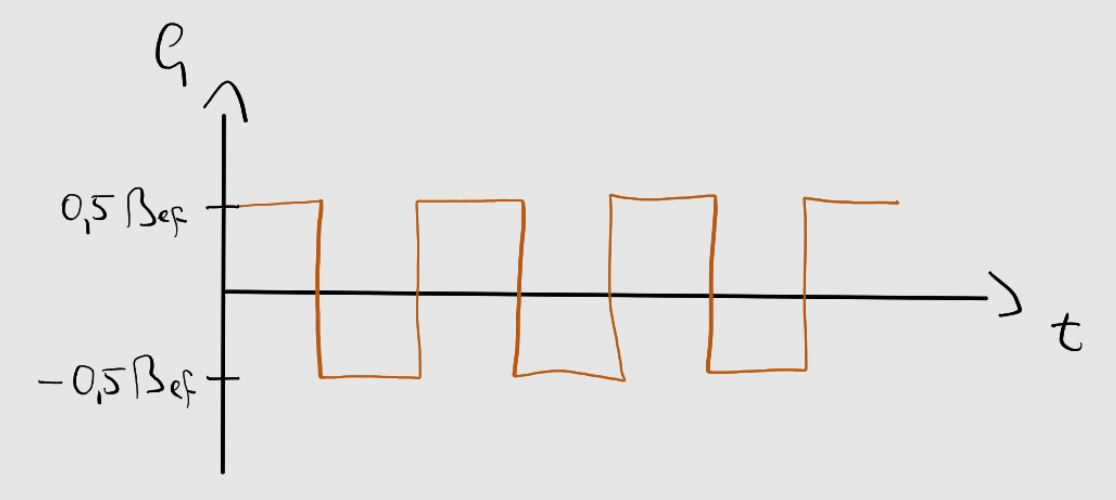
\includegraphics[width=0.5\textwidth]{img/periodicke.jpg}
  \caption{Ukázkový vstup pro periodickou změnu reaktivity.}
  \label{fig_periodicke}
\end{figure}

Poté ale pomocí již zmíněných vztahů pro periody dostáváme:

\begin{itemize}
  \item $+ 0,5 \beta_{\text{ef}} \rightarrow T_e = 10$~s,
  \item $- 0,5 \beta_{\text{ef}} \rightarrow T_e = 100$~s,
\end{itemize}

tedy relativní četnost musí růst rychleji, než klesat. Výsledkem tedy není periodická odezva četnosti, ale četnost postupně roste, viz obrázek \ref{fig_periodicke_reseni}.

\begin{figure}[H]
  \centering
  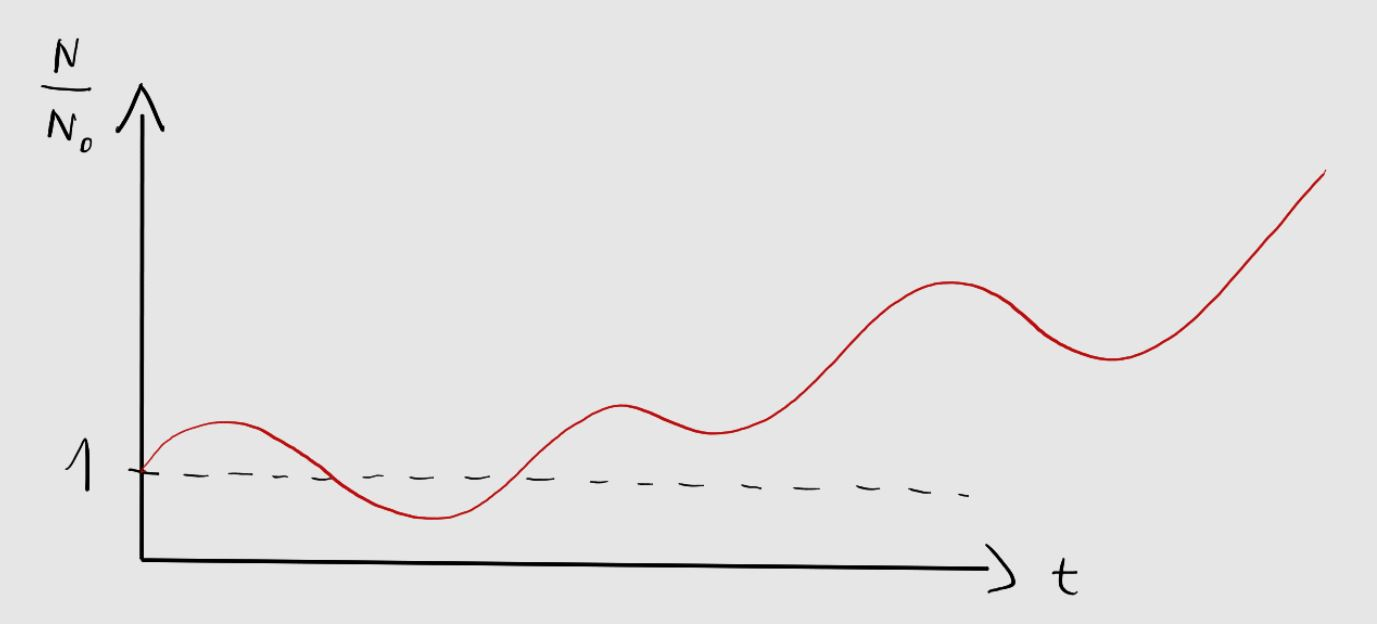
\includegraphics[width=0.5\textwidth]{img/periodicke_reseni.jpg}
  \caption{Ukázkový výstup pro periodickou změnu reaktivity.}
  \label{fig_periodicke_reseni}
\end{figure}

\textbf{Konstantní produkce zpožděných neutronů}

Jde o teoretický model, který lze očekávat v prvních desetinách vteřin po skokové změně reaktivity. Pro odvození opět skočíme do produkčního tvaru, kde předpokládáme, že máme produkční rovnováhu:

$$ \dfrac{dC_i}{dt} |_{0} = 0. $$

Rovnice tedy vypadají:

$$ \dfrac{dN}{dt} = \dfrac{\rho - \beta_{\text{ef}}}{\Lambda} N(t) + \sum_{i=1}^m \lambda_i C_i(t), $$

$$ 0 = -\lambda_i C_i(t) |_{0} + \dfrac{\beta_{\text{ef},i}  N(t)}{\Lambda}. $$

Obě rovnice jsou opět v pohodě řešitelné, ale ani to zde dělat nebudeme\footnote{To bych se musel fakt hodně nudit}. Řešení je ve skriptech a pro konstantní reaktivitu je tvaru:

$$ \dfrac{N(t)}{N_0} = \dfrac{\beta_{\text{ef}}}{\beta_{\text{ef}}-\rho_0} \left [ 1 - \dfrac{\rho_0}{\beta_{\text{ef}}} \exp{ \left ( \dfrac{\rho_0 - \beta_{\text{ef}}}{\Lambda}t \right ) } \right ]. $$

Tímto vztahem je tedy možné popsat průběh do inflexního bodu, který je dán parametrem $C_0$. Je zde možné nalézt paralelu s př. 3, kde se uvažovala pouze jedna skupina zpožděnek. Člen $C_0$ a $C_1$ zde vyšel stejně a exponenciela ve výraze představuje kořen $z_1$. Tato aproximace přibližuje odezvu pouze okamžitých neutronů.\\

Koeficient $C_0$:

$$ C_0 = \dfrac{\beta_{\text{ef}}}{\beta_{\text{eff}} - \rho_0} $$

představuje absolutní hodnotu relativní četnosti neutronů při okamžité změně reaktivity, viz graf na obrázku \ref{fig_konstantni_produkce}.

\begin{figure}[H]
  \centering
  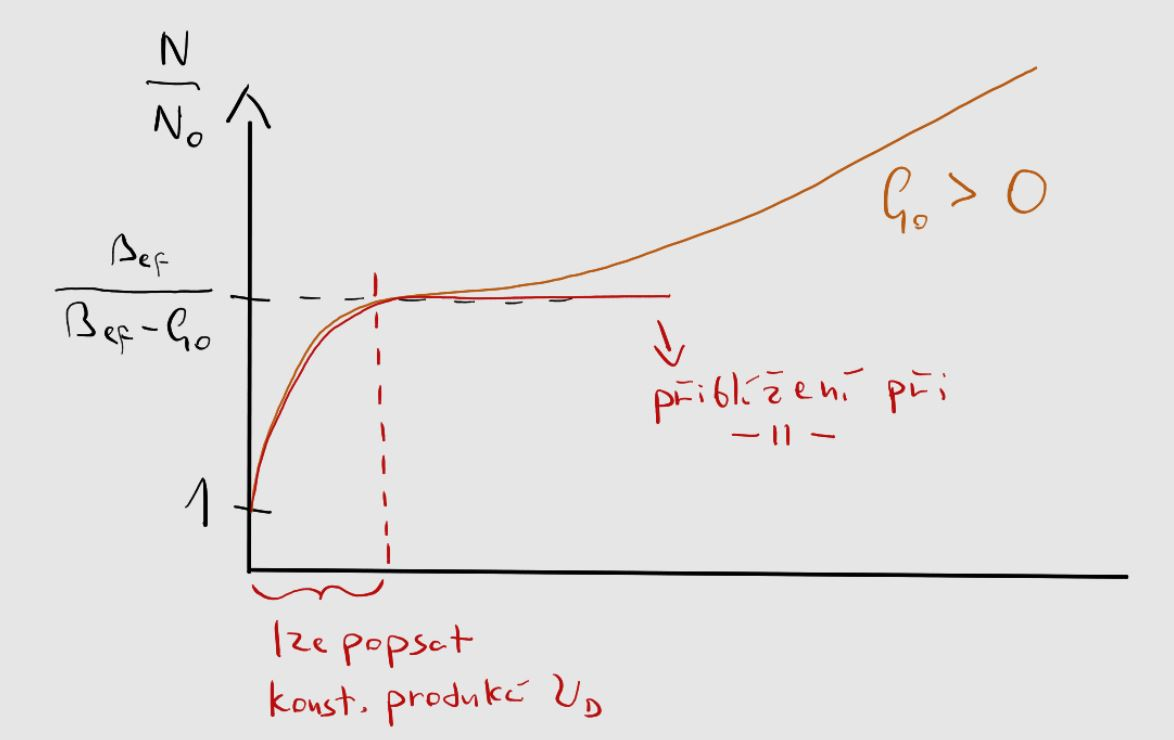
\includegraphics[width=0.5\textwidth]{img/konstantni_produkce.jpg}
  \caption{Průběh relativní četnosti při konstantní produkci zpožděných neutronů (červená křivka) vs. skutečný průběh (oranžová).}
  \label{fig_konstantni_produkce}
\end{figure}

\textbf{Okamžitý skok}

Další možnou aproximací je metoda okamžitého skoku, kdy v čase $t = 0$ předpokládáme:

$$ \dfrac{dN}{dt} = 0. $$

Tuto metodu lze aplikovat až po prvních pár desetinách vteřiny, kdy odezní vliv okamžitých neutronů, tedy v momentě, kdy se nacházíme za inflexním bodem\footnote{Metoda konstantní produkce neutronů se dá použít před inflexním bodem a metoda okamžitého skoku po inflexním bodu.}. Jde o aproximaci přibližující vliv zpožděných neutronů.\\

Následující vztahy jsou odvozeny pouze pro 1 skupinu zpožděných neutronů\footnote{Metoda konstantní produkce zpožděných neutronů vyjadřuje chování v systému díky okamžitým neutronům, proto nebylo potřeba uvažovat různé skupiny zpožděnek. Metoda okamžitého skoku naopak vyjadřuje vliv zpožděných neutronů, ovšem vztahy pro $m$ skupin by byl složitý.} a pro konstantní reaktivitu, přičemž odvození je opět ve skriptech\footnote{To bych se musel fakt hodně nudit.}. Řešíme rovnice tvaru:

$$ 0 = \dfrac{\rho - \beta_{\text{ef}}}{\Lambda} N(t) + \bar{\lambda} C(t), $$

$$ \dfrac{dC}{dt} = -\bar{\lambda} C(t) + \dfrac{\beta_{\text{ef}}  N(t)}{\Lambda}, $$

které dávají řešení:

$$ \dfrac{N(t)}{N_0} = \dfrac{\beta_{\text{ef}}}{\beta_{\text{ef}} - \rho_0} \exp{\left ( \dfrac{\bar{\lambda} \rho_0}{\beta_{\text{ef}} - \rho_0} t \right )}. $$

Je opět možné nalézt paralelu s př. 3, jelikož exponenciála představuje kořen $z_0$ a člen před exponencielou koeficient $C_0$, viz graf na obrázku \ref{fig_okamzity_skok}.

\begin{figure}[H]
  \centering
  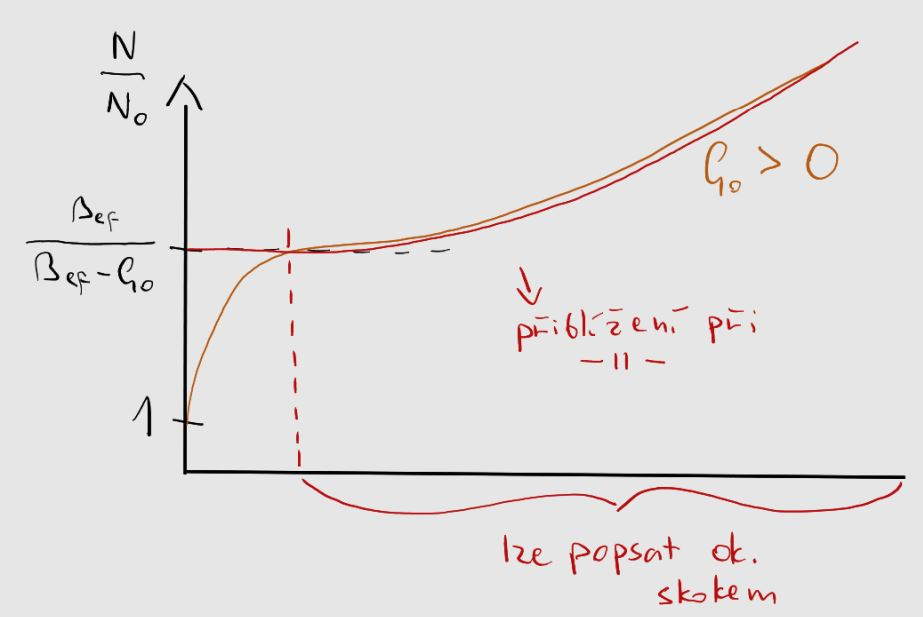
\includegraphics[width=0.5\textwidth]{img/okamzity_skok.jpg}
  \caption{Průběh relativní četnosti při okamžitém skoku (červená křivka) vs. skutečný průběh (oranžová).}
  \label{fig_okamzity_skok}
\end{figure}

Ve skutečnosti je přiblížení jednou skupinou dost mimo a je vhodnější k popisu použít více skupin. Příklad je pouze demonstrační\footnote{Nebo by bylo vhodnější středovat $\bar{\lambda}$ pomocí $\tau_i$.}.\\

\textbf{Externí zdroj neutronů}

Externí zdroj neutronů je dobré využívat k bezpečnějšímu spouštění, jelikož dává silnější tok než pozadí, které umožňuje sledovat kvalitnější odezvu na detektorech\footnote{Pozadí, resp. samoštěpení by šlo ke spuštění použít také, ale bylo by zapotřebí kvalitnější detektory, který by poskytly kvalitní odezvu a spouštění bylo skutečně bezpečné.}. Četnost neutronů při zavedení externího zdroje a pro různé reaktivity systému zobrazuje graf na obrázku \ref{fig_zdroj}.

\begin{figure}[H]
  \centering
  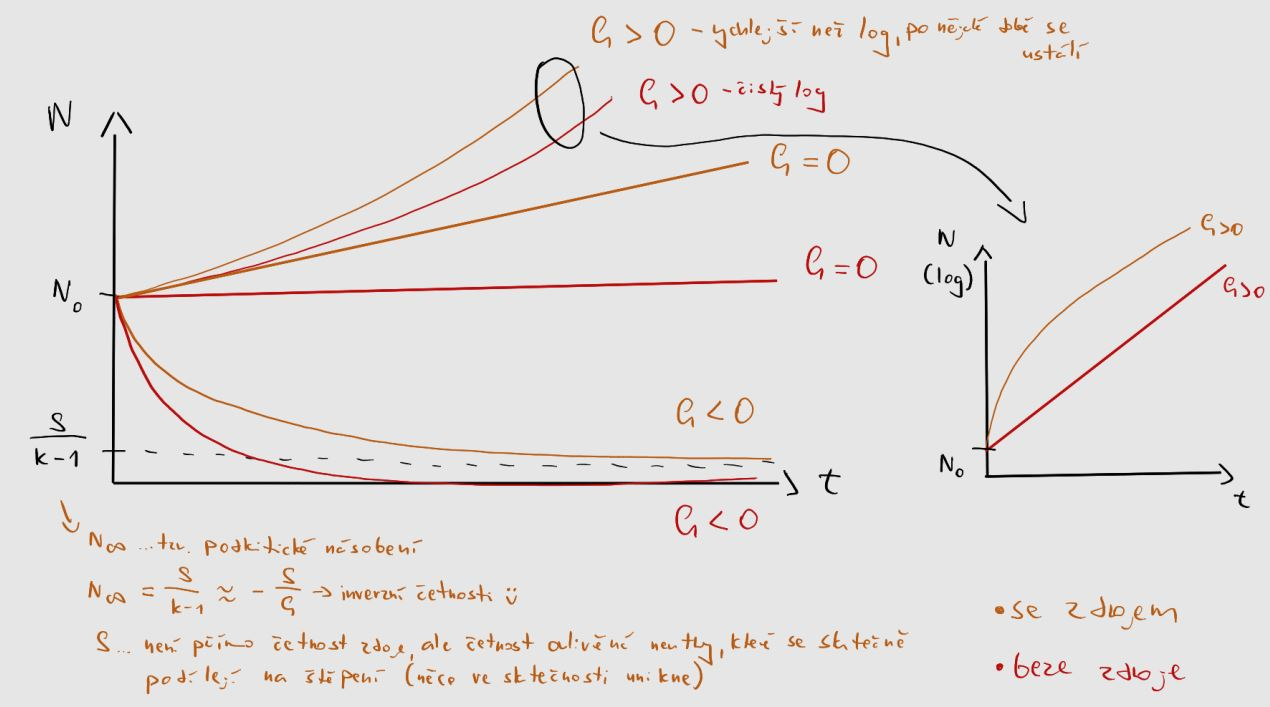
\includegraphics[width=0.8\textwidth]{img/zdroj.jpg}
  \caption{Četnost neutronů pro různé reaktivity s externím zdrojem (oranžová křivka) a bez externího zdroje (červená).}
  \label{fig_zdroj}
\end{figure}

\small

\textbf{Př. 4 -- podmínka stability s externím zdrojem:}

Mějme externí zdroj neutronů a sledujeme, za jakých podmínek se četnost neutronů ustálí. Vyjdeme z produkčního tvaru jednobodové kinetiky (kam dosadíme externí zdroj neutronů $S(t)$) kde předpokládáme ustálený tvar, tedy při dosazení $N(t) = N_0$ a $C_i(t) = C_i^0$ (jde o konstanty $\rightarrow$ nulové derivace) dostáváme tvar:

$$ 0 = \dfrac{\rho(t) - \beta_{\text{ef}}}{\Lambda} N_0 + \sum_{i=1}^m \lambda_i C_i^0 + S(t), $$

$$ 0 = -\lambda_i C_i^0 + \dfrac{\beta_{\text{ef},i}  N_0}{\Lambda}. $$

Rovnice do sebe podosazujeme a dostáváme jednoduché řešení (podmínka stability):

$$ 0 = \dfrac{\rho(t)}{\Lambda} N_0 + S(t). $$

Aby stabilita nastala, musí uvedená rovnice platit. K tomu dojde pouze za předpokladu:

\begin{itemize}
  \item $S(t) = 0$, $\rho(t) = 0$ $\rightarrow$ máme kritický stav a vypnutý zdroj,
  \item $S(t) = 0$, $N_0 = 0$ $\rightarrow$ máme vypnutý reaktor, v praxi zřejmě nedosažitelné,
  \item $S(t) > 0$, $\rho(t) = -S(t) \dfrac{\Lambda}{N_0}$ $\rightarrow$ hledaná podmínka stability pro zapnutý externí zdroj\footnote{Toho jsme využili u metody inverzních četností v ERF, kdy se určovala vnesená reaktivita.}.
\end{itemize}

\textbf{Př. 5 -- vztah mezi dvěmi stavy:}

Nyní předpokládejme, že máme stav s $N_1$, $\rho_1$ a $S_1$, a změnou reaktivity docílíme nového stavu s $N_2$, $\rho_2$ a $S_2$. Zajímá nás vztah mezi $N_1$ a $N_2$ v závislosti na reaktivitách $\rho_{1,2}$ a externích zdrojích $S_{1,2}$. Předpokládejme, že ke změnám došlo okamžitě, proto můžeme aplikovat metodu konstantní produkce zpožděných neutronů i metodu okamžitého skoku (zde si pomůžeme přiblížením $C_i^1(t) = C_i^2(t)$). Schematicky by šel přechod znázornit pomocí grafu na obrázku \ref{fig_podil_N_ukazka}.

\begin{figure}[H]
  \centering
  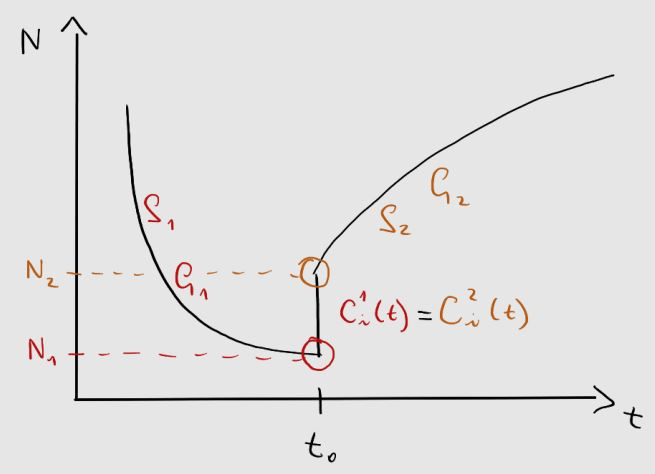
\includegraphics[width=0.5\textwidth]{img/podil_N_ukazka.jpg}
  \caption{Znázornění příkladu pro odvození vztahu mezi dvěmi stavy.}
  \label{fig_podil_N_ukazka}
\end{figure}

Vyjdeme z produkčního tvaru rovnic kinetiky (ale pouze z první rovnice, zpožděnky nás nezajímají), kterou si zapíšeme pro oba stavy a sečteme (obě strany jsou nulové). Dostáváme jednu rovnici:

$$ \dfrac{\rho_1 - \beta_{\text{ef}}}{\Lambda} N_1 + \sum_{i=1}^m \lambda_i C_i(t) + S_1 = \dfrac{\rho_2 - \beta_{\text{ef}}}{\Lambda} N_2 + \sum_{i=1}^m \lambda_i C_i(t) + S_2. $$

Po úpravě a vyjádření získáme:

$$ \dfrac{N_2}{N_1} = \dfrac{\beta_{\text{ef}} - \rho_1}{\beta_{\text{ef}} - \rho_2} + \dfrac{\Lambda}{N_1} \dfrac{S_2 - S_1}{\beta_{\text{ef}} - \rho_2}. $$

Toto přiblížení, přestože je jeho odvození dosti nepřesné a idealistické dává kupodivu přesné výsledky. Předvedeme na pár příkladech.\\

Mějme kritický stav ($\rho_1 = 0$) s externím zdrojem $S_1$. V jistém momentu zdroj vypneme (ve stavu s aktuální četností $N_1$), čímž se dostáváme do stavu s $\rho_2 = 0$ (stále máme kritický stav, četnost ovlivňujeme pouze pomocí zdroje), $S_2 = 0$ a $N_2$. Kupodivu, $N_2$ se neustálí ihned na pozici jako předchozí $N_1$, ale skočí na nižší hladinu, přesně podle rovnice:

$$ \dfrac{N_2}{N_1} = 1 - \dfrac{\Lambda}{N_1} \dfrac{S_1}{\beta_{\text{ef}}}. $$

Tento jev je možné fyzikálně odůvodnit tak, že v momentě vypnutí zdroje vznikají zpožděnky z předchozích generací, kdy ještě četnost nebyla tak vysoká (nižší než ve stavu $N_1$). Je jich tedy výrazně méně a nejsou schopny kompenzovat nedostatek v aktuální generaci, viz obrázek \ref{fig_podil_N_1}.

\begin{figure}[H]
 \centering
 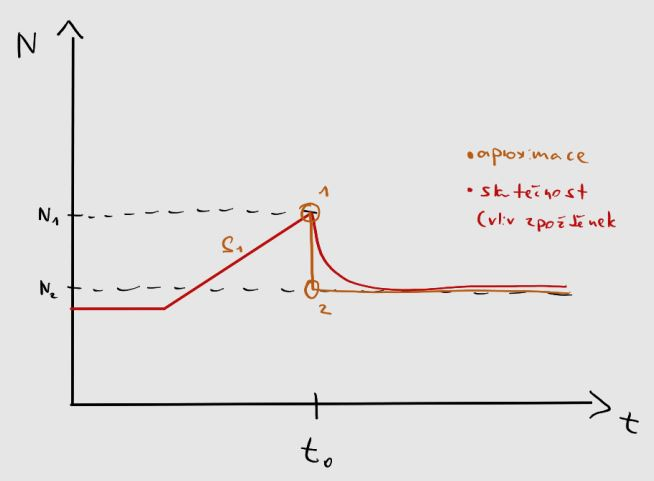
\includegraphics[width=0.6\textwidth]{img/podil_N_1.jpg}
 \caption{První ukázka využití vztahu mezi dvěmi stavy ($S_1$).}
 \label{fig_podil_N_1}
\end{figure}

Dalším příkladem může být zvyšování četnosti pomocí reaktivity. Mějme reaktor bez zdrojů ($S_{1,2} = 0$) a stav s malinkatou reaktivitou $\rho_1$. Opět v jistém momentě s četností $N_1$ vrátíme reaktivitu do stavu $\rho_2 = 0$, přičemž nová četnost opět skokově klesne dle vztahu:

$$ \dfrac{N_2}{N_1} = \dfrac{\beta_{\text{ef}} - \rho_1}{\beta_{\text{ef}}}. $$

Zdůvodnění je zde stejné, viz graf na obrázku \ref{fig_podil_N_2}.

\begin{figure}[H]
 \centering
 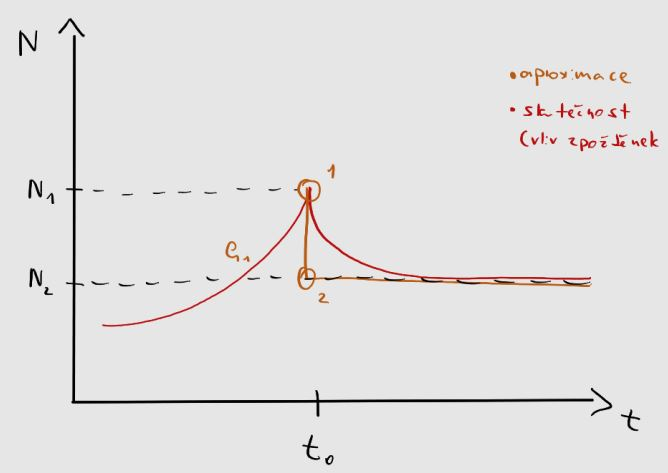
\includegraphics[width=0.6\textwidth]{img/podil_N_2.jpg}
 \caption{Druhá ukázka využití vztahu mezi dvěmi stavy ($\rho_1$).}
 \label{fig_podil_N_2}
\end{figure}

Z praktického hlediska je výhodnější najíždět mezi stavy postupně a nikoliv skokově. Díky tomu nebudeme sledovat skokové změny četností.

\normalsize

\subsubsection{Frekvenční charakteristika}

Pro odvození frekvenční charakteristiky je třeba trochu více matematiky.\\

\textbf{Přenosová funkce nulového reaktoru}

Platí, že každý lineární systém (takový, který je možné popsat soustavou lineárních diferenciálních rovnic) je možné popsat pomocí tzv. \textbf{přenosové funkce nulového reaktoru} $\tilde{W_{yx}}(s)$ definované dle:

\begin{equation}
  \boxed{
  \tilde{W_{yx}}(s) \equiv \dfrac{\tilde{y}(s)}{\tilde{x}(s)},
  \label{prenosova_funkce_definice}}
\end{equation}

kde:

\begin{itemize}
  \item $\tilde{y}(s)$ představuje výstupní veličinu (v našem případě jde o $\tilde{N}(s)$, resp. po převodu $N(t)$),
  \item $\tilde{x}(s)$ představuje vstupní veličinu (v našem případě $\tilde{\rho}(s)$, resp. $\rho(t)$).
\end{itemize}

Poté naši hledanou výstupní funkci nalezneme dle:

$$ \tilde{y}(s) = \tilde{W_{yx}}(s) \cdot \tilde{x}(s). $$

Jedná se o součin dvou Laplaceovsky transformovaných funkcí, tudíž po převedení se jedná o jejich konvoluci:

$$ y(t) = (W_{yx} * x ) (t) = \int_0^t W_{yx}(t-t') x(t') dt'. $$

Pro výpočet potřebujeme znát originální přenosovou funkci, kterou získáme pomocí Laplaceova obrazu\footnote{Ti, co dávali o RMF pozor si všimnou, že se jedná o Greenovu funkci.}:

$$ W_{yx}(t) \equiv \mathcal{L}^{-1}[\tilde{W_{yx}}(s)](t). $$

\textbf{Linearizovaný model}

Jaderný reaktor ale ve skutečnosti není lineárním systémem. Podíváme-li se na rovnici kinetiky v integrálním tvaru (viz \eqref{integralni_kinetika}), všimneme si, že se v integrandu vyskytuje součin vstupní ($\rho(t)$) a výstupní ($N(t)$) veličiny\footnote{Nejde ji napasovat do konvoluce s přenosovou funkcí, kterou jsme si definovali před chvílí.}:

$$ N(t) = N_0 + \int_0^t G_0(t-t') \rho(t') N(t')dt'. $$

Proto musíme rovnici linearizovat. To provedeme, zavedeme-li odchylku $\Delta N(t)$ jako:

$$ \Delta N(t) = N(t) - N_0 $$

a tu dosadíme do integrálního tvaru \eqref{integralni_kinetika}. Výsledkem bude:

$$ \Delta N(t) = N_0 \int_0^t G_0(t-t') \rho(t') dt' + \int_0^t G_0(t-t') \rho(t') \Delta N(t')dt'. $$

Právě ten druhý člen představuje nelinearitu systému. Zavedeme-li předpoklady, že se jedná o malé změny $\rho$ a malé změny $\Delta N$, můžeme druhý člen vypustit a dostaneme linearizovaný tvar:

\begin{equation}
  \boxed{
  \Delta N(t) = N_0 \int_0^t G_0(t-t') \rho(t') dt'.
  \label{linearizovana_kinetika}}
\end{equation}

Podobného výsledku jsme dosáhli už v impulsní charakteristice, ale tam jsme museli předpokládat okamžitý skok pomocí Diracovy funkce. Zde je to o něco málo obecnější a za $\rho(t)$ jde dosazovat víceméně cokoliv.\\

Odtud přejdeme opět zpět k LT pomocí konvoluce a dostáváme:

$$ \Delta \tilde{N}(s) = N_0 \tilde{G_0}(s) \tilde{\rho} (s), $$

což pokud chceme dokázat, že se jedná o lineární systém, chceme dostat do stejného tvaru, jako jsme si definovali přenosovou funkci nulového reaktoru (výstupní/vstupní). Zároveň za $\tilde{G_0}(s)$ můžeme dosadit z definice \eqref{prenosova_funkce}, čímž dostaneme:

$$ \tilde{G_0}(s) = \dfrac{1}{N_0} \dfrac{\Delta \tilde{N}(s)} {\tilde{\rho}(s)} = \dfrac{1}{s \left ( \Lambda + \sum_{i=1}^m \dfrac{\beta_{\text{ef},i}}{\lambda_i + s} \right )}.$$

\textbf{Frekvenční charakteristika -- konečně}

Nyní můžeme konečně řešit frekvenční charakteristiku, tedy předpoklad, že máme periodicky se měnící reaktivitu:

$$ \rho(t) = \rho_0 \cos (\omega t), $$

což v LT znamená:

$$ \tilde{\rho}(s) = \dfrac{s}{s^2 + \omega^2}. $$

Zajímá nás relativní změna četnosti, tedy:

$$ \dfrac{\Delta \tilde{N}(s)}{N_0} = \tilde{\rho}(s) \tilde{G_0}(s) = \rho_0 \: \dfrac{s}{s^2 + \omega^2} \: \dfrac{1}{s \left ( \Lambda + \sum_{i=1}^m \dfrac{\beta_{\text{ef},i}}{\lambda_i + s} \right )} = \rho_0 \: \dfrac{1}{s^2 + \omega^2} \: \dfrac{1}{\Lambda + \sum_{i=1}^m \dfrac{\beta_{\text{ef},i}}{\lambda_i + s}}. $$

Jde opět o lomenný výraz, tudíž ho můžeme převést na parciální zlomky\footnote{Nyní opět použijeme koeficienty $A_n$ a kořeny $s_n$, jelikož je tu jistá paralela s impulsní charakteristikou.}. Výraz má celkem $m+2$ kořenů. Prvních $m$ známe, jsou to ty záporné z impulsní charakteristiky. Zbylé dva kořeny jsou imaginární\footnote{Jako imaginární jednotku značíme $j$.}:

\begin{itemize}
  \item $s_n < 0 \: \: \: \forall \: n \in \widehat{m}$, navíc jsou stejné jako v impulsní charakteristice,
  \item $s_{m+1} = \omega j$,
  \item $s_{m+2} = - \omega j$.
\end{itemize}

Podle kuchařky dostaneme celkové řešení tvaru:

$$ \dfrac{\Delta \tilde{N}(s)}{N_0} = \sum_{n = 1}^{m+2} \dfrac{A_n}{s-s_n}, $$

$$ \dfrac{\Delta N(t)}{N_0} = \sum_{n = 1}^{m+2} A_n e^{s_n t}. $$

Díky zápornosti prvních $m$ členů první členy po čase vymizí a zůstanou pouze členy $m+1$ a $m+2$. Jejich kořeny jsou ryze imaginární $\rightarrow$ vede na řešení v goniometrických funkcích. Po trošce matematiky (substituci $s = \omega j$ a předpokladu\footnote{Resp. znalosti, prý to tak fakt je.}, že $\tilde{G_0}(\omega j)$ je komplexně sdružená funkce) dostaneme vyjádření koeficientů $A_{m+1}$ a $A_{m+2}$:

$$ A_{m+1} = \dfrac{\rho_0}{2} \tilde{G_0}(\omega j), $$
$$ A_{m+2} = \dfrac{\rho_0}{2} \tilde{G_0}(-\omega j), $$

tedy:

$$ \dfrac{\Delta N(t)}{N_0} \approx = \rho_0 \left [\dfrac{1}{2} \tilde{G_0}(\omega j) e^{\omega j t} + \dfrac{1}{2} \tilde{G_0}(-\omega j) e^{-\omega j t} \right ], $$

což je ve finále možné vyjádřit pomocí fázového posuvu $\varphi$:

\begin{equation}
  \boxed{
  \dfrac{\Delta N(t)}{N_0} = \rho_0 | \tilde{G_0}(\omega j) | \cos (\omega t + \varphi),
  \label{frekvencni_charakteristika_reseni}}
\end{equation}

kde pro $\varphi$ platí:

\begin{equation}
  \boxed{
  \varphi = \text{arctg} \left ( \dfrac{\text{Im} (\tilde{G_0}(\omega j)}{\text{Re}(\tilde{G_0}(\omega j)} \right ).
  \label{frekvencni_charakteristika_faze}}
\end{equation}

Co to tedy znamená? Máme-li periodickou změnu reaktivity, tak dostáváme periodickou odezvu na četnosti, která je ovšem posunutá o fázový posuv $\varphi$, viz graf na obrázku \ref{fig_frekvencni}.\\

\begin{figure}[H]
 \centering
 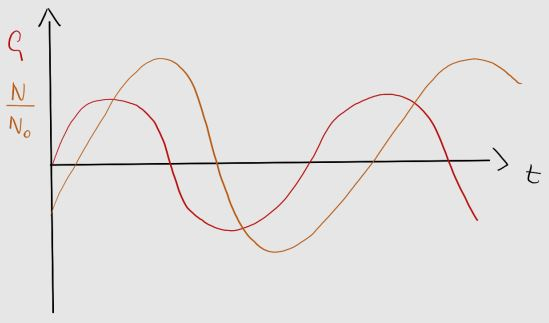
\includegraphics[width=0.6\textwidth]{img/frekvencni.jpg}
 \caption{Závislost relativní změny četnosti neutronů pro frekvenční charakteristiku a fázový posuv mezi odezvou a změnou reaktivity.}
 \label{fig_frekvencni}
\end{figure}

Absolutní hodnota je závislá pouze na frekvenci $\omega$ a vlastnostech reaktoru ($\Lambda$, $\lambda_i$ atd.). Ve skutečnosti ale maximální hodnota četnosti roste (viz obrázek \ref{fig_periodicke_reseni}). Tato nesrovnalost je způsobena právě linearizací systému. Toto přiblížení je tedy možné použít pouze pro kratší časy nebo menší reaktivity, kdy se nestihne rozvinout exponenciální odezva.\\

Pokud by nás zajímalo, jak vypadá závislost mezi frekvencí a aplitudou, resp. fázovým posuvem, stačí se juknout na graf na obrázku \ref{fig_frekvencni_zavislost}.

\begin{figure}[H]
  \centering
  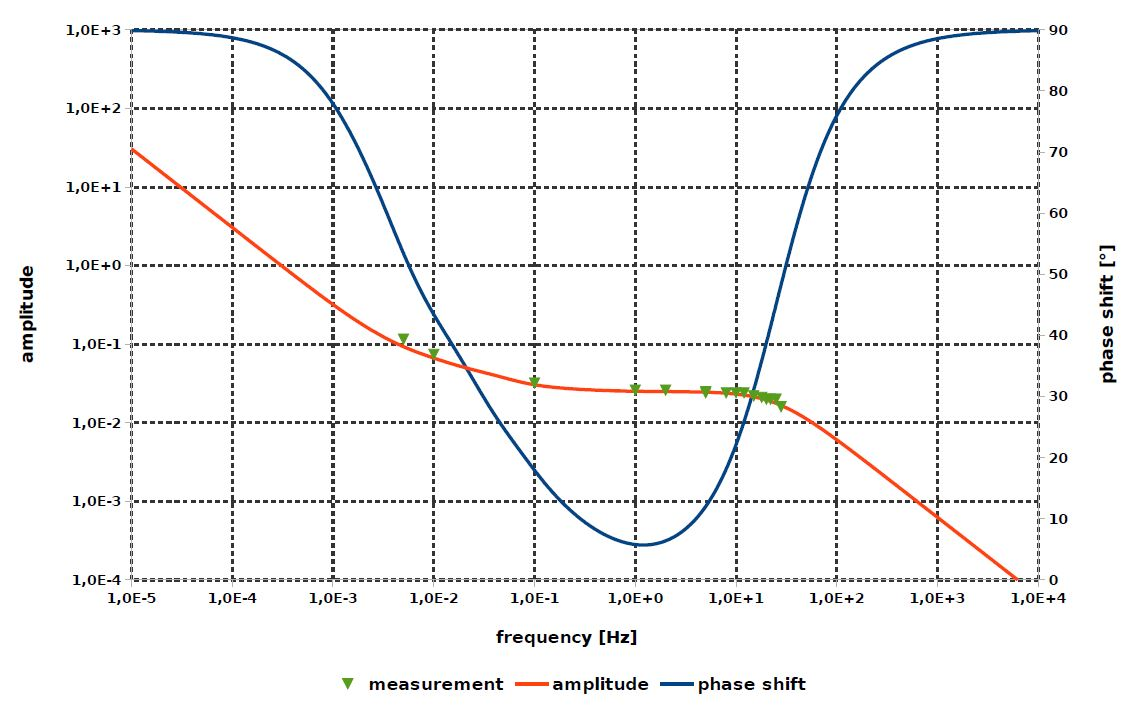
\includegraphics[width=1\textwidth]{img/frekvencni_zavislost.jpg}
  \caption{Závislost mezi frekvencí a amplitudou, resp. fázovým posuvem u frekvenční charakteristiky.}
  \label{fig_frekvencni_zavislost}
\end{figure}

Důkaz pro závislost amplitudy (která je ovlivněna $|\tilde{G_0}(\omega)|$) zde:\\

\textbf{a) Oblast pomalých změn:}

Tedy oblast s malými $\omega$, tedy i s malými $s$. V takovém případě můžeme v přenosové funkci zanedbat $s$ ve zlomku v sumě:

$$ \tilde{G_0}(s) = \dfrac{1}{s \left ( \Lambda + \sum_{i=1}^m \dfrac{\beta_{\text{ef},i}}{\lambda_i + s} \right )} \approx \dfrac{1}{s \left ( \Lambda + \sum_{i=1}^m \dfrac{\beta_{\text{ef},i}}{\lambda_i} \right )} = \dfrac{1}{s \ell^*} = \dfrac{1}{j \omega \ell^*} = - \dfrac{j}{\omega \ell^*}. $$

Tedy pro amplitudu:

$$ |\tilde{G_0}(\omega)| = \dfrac{1}{\omega \ell^*}. $$

A speciální případ (kvůli grafu):

$$ \left |\tilde{G_0} \left ( \dfrac{\beta_{\text{ef}}}{\ell^*} \right ) \right | = \dfrac{1}{\beta_{\text{ef}}}. $$

\textbf{b) Oblast rychlých změn:}

Zde můžeme ze stejného zlomku odstranit $\lambda_i$, potom dostaneme:

$$ \tilde{G_0}(s) = \dfrac{1}{s \left ( \Lambda + \sum_{i=1}^m \dfrac{\beta_{\text{ef},i}}{\lambda_i + s} \right )} \approx \dfrac{1}{s \left ( \Lambda + \sum_{i=1}^m \dfrac{\beta_{\text{ef},i}}{s} \right )} = \dfrac{1}{s \ell} = \dfrac{1}{j \omega \ell} = - \dfrac{j}{\omega \ell}. $$

Speciální případ:

$$ \left |\tilde{G_0} \left ( \dfrac{\beta_{\text{ef}}}{\ell} \right ) \right | = \dfrac{1}{\beta_{\text{ef}}}. $$

\textbf{c) Oblast středně rychlých změn:}

Zde můžeme\footnote{Z neznámých důvodů.} odstranit z výrazu $\Lambda$ a dostaneme:

$$ \tilde{G_0}(s) = \dfrac{1}{s \left ( \Lambda + \sum_{i=1}^m \dfrac{\beta_{\text{ef},i}}{\lambda_i + s} \right )} \approx \dfrac{1}{s \left ( \sum_{i=1}^m \dfrac{\beta_{\text{ef},i}}{\lambda_i + s} \right )} = \dfrac{1}{\sum_{i=1}^m \dfrac{\beta_{\text{ef},i}}{1 + \dfrac{\lambda_i}{s}} }. $$

Za předpokladu, že $\dfrac{\lambda_i}{s} \rightarrow 0$ dostáváme:

$$ \left |\tilde{G_0} \left (\omega \right ) \right | = \dfrac{1}{\beta_{\text{ef}}}. $$

Sumasumárum, závislost amplitudy na frekvenci (spočtenou vs. skutečnou) zobrazuje graf na obrázku \ref{fig_amplituda_frekvence}.

\begin{figure}[H]
  \centering
  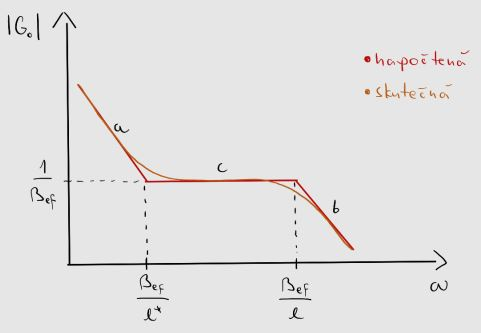
\includegraphics[width=0.6\textwidth]{img/amplituda_frekvence.jpg}
  \caption{Spočtená (červená) vs. napočtená (oranžová) závislost amplitudy na frekvenci při frekvenční charakteristice.}
  \label{fig_amplituda_frekvence}
\end{figure}

\subsubsection{Vlivy zjendnodušení}

Na závěr se podíváme, v jakých oblastech změn reaktivity můžeme použít různá zjednodušení v rovnicích jednobodové kinetiky.


\textbf{Zanedbání zpožděnek}

Zajímá nás, v jaké oblasti funguje jednobodová kinetika při zanedbání zpožděných neutronů. Dosadíme odchylku $\Delta N(t)$ do rovnice bodové kinetiky a s jediným zanedbáním malé změny reaktivity:

$$ \dfrac{d (\Delta N)}{dt} = \dfrac{k_{\text{ef}}-1}{\ell} (N_0 + \Delta N) \doteq \dfrac{\rho}{\ell} N_0. $$

Rovnici zLaplaceujeme a dostaneme:

$$ \tilde{\Delta N} = \dfrac{N_0}{\ell} \dfrac{\tilde{\rho}}{s}. $$

Dosadíme do definice přenosové funkce:

$$ \tilde{G_0}(s) = \dfrac{\tilde{\Delta N}}{N_0 \rho} = \dfrac{1}{s \ell}. $$

Toto je v podstatě to samé, co jsme získali v oblasti rychlých změn frekvenční charakteristiky. To tedy znamená, že toto přiblížení (bez zpožděnek) platí právě pro oblast rychlých změn reaktivity.\\

\textbf{Efektivní doba života neutronů}

Co se stane, pokud zaměníme $\ell$ za $\ell^*$? Odvození stejné, pouze dosadím nakonec $\ell^*$, zjednodušení tedy platí v oblasti pomalých změn reaktivity.\\

\textbf{Konstantní produkce zpožděnek}

V takovém případě je možné popsat systém pomocí jedné rovnice:

$$ \dfrac{dN}{dt} = \dfrac{\rho(t) - \beta_{\text{ef}}}{\Lambda} N(t) + \dfrac{\beta_{\text{ef}}}{\Lambda} N_0. $$

Stejným způsobem zavedeme odchylky a zlinearizujeme

$$ \dfrac{d (\Delta N)}{dt} = \dfrac{\rho(t)}{\Lambda} P_0 - \dfrac{\beta_{\text{ef}}}{\Lambda} \Delta N. $$

Zlaplaceujeme, dosadíme opět do přenosové funkce a máme:

$$ \tilde{G_0} (s) = \dfrac{1}{\Lambda s +  \beta_{\text{eff}}}. $$

Tento vztah je možné získat i z přímé definice přenosové funkce, při $\lambda_i \rightarrow 0$. Toto zjednodušení platí v oblasti rychlých a částečně rychlých změn.\\

\textbf{Okamžitý skok}

Složitá rovnice, vynecháme. Ve výsledku dostaneme:

$$ \tilde{G_0} (s) = \dfrac{s+\bar{\lambda}}{s \beta_{\text{eff}}}. $$

Toto je možné použít v oblasti malých změn a pomalých přechodových procesech.



\subsection{Numerické řešení s vlivem zpožděných neutronů}

K numerickému řešení rovnic jednobodové kinetiky se využívá kombinace několika numerických metod. Každé numerické řešení je zatíženo několika chybami. Ty můžeme obecně řadit do dvou kategorií:

\begin{itemize}
  \item \textbf{Truncation error} -- chyby diskretizace (vznikají díky diskretizaci obecně spojitých funkcí a předpisů),
  \item \textbf{Round-off error} -- chyby zaokrouhlování (vznikají díky konečnému výčtu čísel při zápisu v PC).
\end{itemize}

Zakreslíme-li graf závislosti chyby na velikosti kroku $h$ (který používáme právě k diskretizaci), zjistíme, že průběh odpovídá cca grafu na obrázku \ref{fig_error}. Při jisté volbě kroku lze nalézt minimum chyby, které se při řešení dopustíme. Rozhodně tedy neplatí, že čím menší krok, tím menší chyba!

\begin{figure}[H]
 \centering
 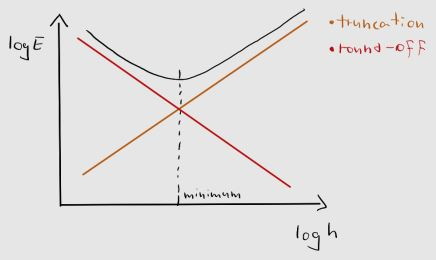
\includegraphics[width=0.6\textwidth]{img/error.jpg}
 \caption{Závislost mezi zvoleným krokem a chybou numerické metody.}
 \label{fig_error}
\end{figure}

\subsubsection{Metoda tečen}

První možností je využít numerické metody pouze ke hledání kořenů $s_n$, resp. $z_n$ v obecném analytickém vyjádření ve formě sumy exponenciel. Koeficienty $A_n$, resp. $C_n$ je poté jednoduché určit dle kuchařky. V takovém případě se může využít metoda půlení intervalu, či právě \textbf{metoda tečen}.\\

U metody tečen se využívá numerické derivace:

$$ y'_i \doteq \dfrac{\Delta y}{\Delta x} = \dfrac{y_{i+1}-y_i}{x_{i+1}-x_i}. $$

Při volbě počátečního odhadu $(x_i, y_i)$ hledáme takové $x_{i+1}$, pro které platí, že $y_{i+1} = 0$, tedy:

$$ x_{i+1} = x_i - \dfrac{y_i}{y'_i}. $$

Hodnotu $y'_i$ zjistíme pomocí Eulerovy dopředné metody, či pomocí Runge-Kutteovy metody (viz dále). Takto se posuneme o další krok a proces opakujeme do té doby, než je relativní odchylka menší než dané $\varepsilon$.\\

\small

\textbf{Př. 6 -- Metoda tečen v přechodové charakteristice}

Pro hledání kořenů $z_n$ vyjdeme z rovnice:

$$ z \left ( \Lambda + \sum_{i = 1}^m \dfrac{\beta_{\text{ef},i}}{z + \lambda_i} \right ) - \rho_0 = 0. $$

Při trochu bastlení, programování a vzpomínání na pana Valentu dáme dohromady celý skript, který vyplyvne správně nalezené kořeny. Poté vytáhneme kuchařku, vyplodíme koeficienty $C_n$ a průběh vykreslíme, viz obrázek XX - DOPLNIT!.

\normalsize

\subsubsection{Eulerova metoda}

Eulerova metoda představuje numerickou derivaci, která vychází z Taylorovy řady. Platí totiž:

$$ y_{i+1} = y_i + y'_i h + \dfrac{y''_i}{2!} h^2 + ... + \dfrac{y^{(n)}_i}{n!} h^n + \mathcal{O}(n). $$

Při troše představivosti:

\begin{itemize}
  \item \textbf{Eulerova dopředná metoda:} $y_{i+1} = y_i + y'_i h$
\end{itemize}

\subsection{Stabilita nulového reaktoru}

Stabilitu je možné ověřit pomocí podmínky:

$$ \int_0^\infty  |G_0(t)| dt < \infty. $$

Nulový reaktor ale není stabilní systém, jelikož integrál nekonverguje. Ve skutečnosti se ale začínají při rostoucím výkonu ozývat zpětné vazby $\rightarrow$ dynamika reaktoru. Reaktory se zápornou zpětnou vazbou jsou stabilní.
